\documentclass{article}

% Language setting
% Replace `english' with e.g. `spanish' to change the document language
\usepackage[english]{babel}

% Set page size and margins
% Replace `letterpaper' with`a4paper' for UK/EU standard size
\usepackage[letterpaper,top=2cm,bottom=2cm,left=3cm,right=3cm,marginparwidth=1.75cm]{geometry}

% Useful packages
\usepackage{amsmath}
\usepackage{amssymb}
\usepackage{mathtools}
\usepackage{graphicx}
\usepackage[colorlinks=true, allcolors=blue]{hyperref}

\usepackage{hyperref}
\hypersetup{
    colorlinks=true,
    linkcolor=blue,
    filecolor=magenta,      
    urlcolor=cyan,
    pdftitle={Overleaf Example},
    pdfpagemode=FullScreen,
    }

\urlstyle{same}

\usepackage{tikz-cd}

%%%%%%%%%%% Box pacakges and definitions %%%%%%%%%%%%%%
\usepackage[most]{tcolorbox}
\usepackage{xcolor}

% Define the colors
\definecolor{boxheader}{RGB}{0, 51, 102}  % Dark blue
\definecolor{boxfill}{RGB}{173, 216, 230}  % Light blue

% Define the tcolorbox environment
\newtcolorbox{mathdefinitionbox}[2][]{%
    colback=boxfill,   % Background color
    colframe=boxheader, % Border color
    fonttitle=\bfseries, % Bold title
    coltitle=white,     % Title text color
    title={#2},         % Title text
    enhanced,           % Enable advanced features
    attach boxed title to top left={yshift=-\tcboxedtitleheight/2}, % Center title
    boxrule=0.5mm,      % Border width
    sharp corners,      % Sharp corners for the box
    #1                  % Additional options
}
%%%%%%%%%%%%%%%%%%%%%%%%%

\newtcolorbox{dottedbox}[1][]{%
    colback=white,    % Background color
    colframe=white,    % Border color (to be overridden by dashrule)
    sharp corners,     % Sharp corners for the box
    boxrule=0pt,       % No actual border, as it will be drawn with dashrule
    boxsep=5pt,        % Padding inside the box
    enhanced,          % Enable advanced features
    overlay={\draw[dashed, thin, black, dash pattern=on \pgflinewidth off \pgflinewidth, line cap=rect] (frame.south west) rectangle (frame.north east);}, % Dotted line
    #1                 % Additional options
}

\usepackage{biblatex}
\addbibresource{sample.bib}


%%%%%%%%%%% New Commands %%%%%%%%%%%%%%
\newcommand*{\T}{\mathcal T}
\newcommand*{\cl}{\text cl}


\newcommand{\ket}[1]{|#1 \rangle}
\newcommand{\bra}[1]{\langle #1|}
\newcommand{\inner}[2]{\langle #1 | #2 \rangle}
\newcommand{\R}{\mathbb{R}}
\newcommand{\C}{\mathbb{C}}
\newcommand{\V}{\mathbb{V}}
\newcommand{\Hilbert}{\mathcal{H}}
\newcommand{\oper}{\hat{\Omega}}
\newcommand{\lam}{\hat{\Lambda}}
\newcommand{\defeq}{\vcentcolon=}

\newcommand{\bigslant}[2]{{\raisebox{.2em}{$#1$}\left/\raisebox{-.2em}{$#2$}\right.}}
\newcommand{\restr}[2]{{% we make the whole thing an ordinary symbol
  \left.\kern-\nulldelimiterspace % automatically resize the bar with \right
  #1 % the function
  \vphantom{\big|} % pretend it's a little taller at normal size
  \right|_{#2} % this is the delimiter
  }}
%%%%%%%%%%%%%%%%%%%%%%%%%%%%%%%%%%%%%%%


\tcbset{theostyle/.style={
    enhanced,
    sharp corners,
    attach boxed title to top left={
      xshift=-1mm,
      yshift=-4mm,
      yshifttext=-1mm
    },
    top=1.5ex,
    colback=white,
    colframe=blue!75!black,
    fonttitle=\bfseries,
    boxed title style={
      sharp corners,
    size=small,
    colback=blue!75!black,
    colframe=blue!75!black,
  } 
}}

\newtcbtheorem[number within=section]{Theorem}{Theorem}{%
  theostyle
}{thm}

\newtcbtheorem[number within=section]{Definition}{Definition}{%
  theostyle
}{def}



\title{Math 214 Homework 1}
\author{Keshav Balwant Deoskar}

\begin{document}
\maketitle

% \vskip 0.5cm


%%%%%%%%%%%%%%%%%%%%%%%%%%%%%%%%%%%%%%%%%%%%%%%%%%%%%%%%%%%%%%%%%
\textbf{Q1.} Let $(X_1, d_1), (X_2, d_2)$ be two metric spaces with the standard topologies induced by their metrics. Show that $f : X_1 \rightarrow X_2$ is continuous as a map between topological spaces if and only if it is continuous in the $\epsilon - \delta$ sense as a map between metric spaces.
%%%%%%%%%%%%%%%%%%%%%%%%%%%%%%%%%%%%%%%%%%%%%%%%%%%%%%%%%%%%%%%%%

\vskip 0.5cm
\textbf{Proof:} 

\begin{itemize}
  \item $\implies$ direction: Fix a point $f(x_0) \in X_2$ and for some $\epsilon > 0$ suppose we have another point $f(x) \in X_2$ so that  $d_2((x), f(x_0)) < \epsilon$. We want to show there exists $\delta > 0$ such that $d_1(x, x_0) < \delta$.
  \vskip 0.25cm
  
  Since $f$ is open in terms of topologies, the pre-image of the open ball $B \defeq B_{\epsilon}(f(x_0)) \subseteq X_2$ is open in $X_1$. That is, $f^{-1}(B) \subseteq X_1$ is open. Further, since both $f(x), f(x_0) \in B$ we know that $x, x_0 \in f^{-1}(B)$. So, we can set $\delta = \sup \{ d(a, b) : a, b \in f^{-1}(B) \}$. This gives us continuity in the $\epsilon-\delta$ sense.

  \vskip 0.5cm
  \item $\impliedby$ direction: We need to show, using $\epsilon-\delta$ continuity, that every open set in $X_2$ has open pre-image in $X_1$. In a metric space, open sets are generated by the basis formed by \textbf{open balls}, so it suffices to show the above holds for an open ball of arbitrary radius.
  
  \vskip 0.25cm
  Consider the open $\epsilon-$ball $B \defeq B_{\epsilon}(f(x_0))$ centered around a point $f(x_0) \in X_2$ for some $\epsilon > 0$. We need to show that $f^{-1}(B)$ is open in $X_1$.

  Choose some other point $f(x) \in B$. Then, since $d_2(f(x), f(x_0)) < \epsilon$. By the hypothesis, we know $d_1 (x, x_0) < \delta_x$ for some $\delta_x > 0$. So, letting $\delta = \frac{1}{2} \delta_x$, certainly we have 
  \[ \underbrace{B_{\delta}(x)}_{\text{open in }X_1} \subset f^{-1}(B) \]

  This argument works for any point $x \in f^{-1}(B)$, so every element of $f^{-1}(B)$ is an interior point. This shows the pre-image, $f^{-1}(B)$, of an open ball $B$ is also open. As a result, any the pre-image of any open subset of $X_2$ is open in $X_1$.
\end{itemize}
\vskip 0.5cm
\hrule 

\vskip 0.5cm

%%%%%%%%%%%%%%%%%%%%%%%%%%%%%%%%%%%%%%%%%%%%%%%%%%%%%%%%%%%%%%%%%
\textbf{Q2.} Let $(X, \mathcal{O}_X)$ be a topological space and $Y \subset X$ a subset. Show that the subspace topology $\mathcal{O}_Y$ is the coarsest topology with respect to which the inclusion map $Y \hookrightarrow X$ is continuous (i.e. that if $\mathcal{O}'$ is another topology on $Y$ such that $Y \hookrightarrow X$ is continuous, then $\mathcal{O}_Y \subset \mathcal{O}$).
%%%%%%%%%%%%%%%%%%%%%%%%%%%%%%%%%%%%%%%%%%%%%%%%%%%%%%%%%%%%%%%%%

\vskip 0.5cm
\textbf{Proof:} Let's denote the coarsest topology on $Y$ such that the inclusion $i : Y \rightarrow X$ is continuous as 
\[ \tau = \{ i^{-1}(V) : V \in \mathcal{O}_X \} \]

\begin{dottedbox}
  Why is $\tau$ the coarsest topology on $Y$?

  \vskip 0.25cm
  By definition, the inclusion is continuous if and only if $i^{-1}(V)$, for all $V \in \mathcal{O}_X$. So, if $\sigma$ is a topology on $Y$, at the very least we must have 
  \[ \{ i^{-1}(V) : V \in \mathcal{O}_X \} \subset \sigma \]
\end{dottedbox}

Now, the subspace  topology is defined as the collection
\[ \mathcal{O}_Y = \{ V \subseteq Y \;|\; V = U \cap Y, \;\;U \in \mathcal{O}_X \}\]

We want to show that $\tau = \mathcal{O}_Y$ i.e. 
\[ \{ i^{-1}(V) : V \in \mathcal{O}_X \} = \{ V \subseteq Y \;|\; V = U \cap Y, \;\;U \in \mathcal{O}_X \} \]

\vskip 0.25cm
For any $V \subseteq X$, consider $v \in V$. Then, since $i^{-1}$ is a function from $X$ to $Y$, if $v \in Y$ then it gets mapped to itself. Otherwise, it gets mapped into the empty set. Thus, clearly, we have 
\[ i^{-1}(V) = V \cap Y \]
so the two topologies are equal.

\vskip 0.25cm
Thus, the subspace topology is the coarsest topology such that the inclusion map in continuous.


\vskip 0.5cm
\hrule 
\vskip 0.5cm

%%%%%%%%%%%%%%%%%%%%%%%%%%%%%%%%%%%%%%%%%%%%%%%%%%%%%%%%%%%%%%%%%
\textbf{Q3.} Let $X$ and $Y$ be two topologcal spaces and let $X' \subset X$, $Y' \subset Y$ be subspaces equipped with the subspace topology. Let $f : X \rightarrow Y$ be a continuous function such that $f(X') \subset Y$. Show that $\restr{f}{X'} : X' \rightarrow Y'$ is continuous.
%%%%%%%%%%%%%%%%%%%%%%%%%%%%%%%%%%%%%%%%%%%%%%%%%%%%%%%%%%%%%%%%%

\vskip 0.5cm
\textbf{Proof:} 

Consider an open set $U \subseteq Y'$. Then, we can write $U = V \cap Y'$ for $V$ open in $Y$. 
\begin{align*}
  \restr{f}{X'}^{-1}(U) &= \restr{f}{X'}^{-1}(V \cap Y') \\
  &= \left( \restr{f}{X'}^{-1}(V) \right) \cap \left( \restr{f}{X'}^{-1}(Y') \right) \;\;\text{  (By elementary set theory)} \\
  &= \left(f^{-1}(V) \cap X'\right) \cap \left(f^{-1}(Y') \cap X'\right) \\
  &= \tilde{V} \cap \tilde{Y'}
\end{align*}


and this is open since it is a finite intersection of $\tilde{V} = f^{-1}(V) \cap X'$ and $\tilde{Y'} = f^{-1}(Y') \cap X'$ which are both open in $X'$ with respect to the subspace topology.

\vskip 0.5cm
\hrule 
\vskip 0.5cm

%%%%%%%%%%%%%%%%%%%%%%%%%%%%%%%%%%%%%%%%%%%%%%%%%%%%%%%%%%%%%%%%%
\textbf{Q4.} Let $X$ be a topological space with the property that for any $p, q \in X$ with $p \neq q$ there is a continuous function $f : X \rightarrow \mathbb{R}$ such that $f(p) \neq f(q)$. Show that this implies $X$ is Hausdorff.
%%%%%%%%%%%%%%%%%%%%%%%%%%%%%%%%%%%%%%%%%%%%%%%%%%%%%%%%%%%%%%%%%

\vskip 0.5cm
\textbf{Proof:} 

Since $f(p) \neq f(q)$, the distance $d = \frac{|p - q|}{3}$ is non-zero. Consider the open balls $B_1 \defeq B_d(f(p))$ and $B_2 \defeq B_d(f(q))$. Clearly, $B_1 \cap B_2 = \emptyset$, so their pre-images are also disjoint.

Now since $f$ is continuous, their preimages $f^{-1}(B_1)$ and $f^{-1}(B_2)$ are open in $X$. Thus, we have found disjoint open sets for each of the points $x$, $y$. The space $X$ is Hausdorff.
\vskip 0.5cm
\hrule 
\vskip 0.5cm

%%%%%%%%%%%%%%%%%%%%%%%%%%%%%%%%%%%%%%%%%%%%%%%%%%%%%%%%%%%%%%%%%
\textbf{Q5.} Let $X$ be a Hausdorff topological space and let $Y \subset X$ be a subset with the subspace topology. Show that $Y$ is Hausdorff.
%%%%%%%%%%%%%%%%%%%%%%%%%%%%%%%%%%%%%%%%%%%%%%%%%%%%%%%%%%%%%%%%%

\vskip 0.5cm
\textbf{Proof:} 
Consider points $p, q \in Y \subset X$. Since $X$ is Hausdorff, there exist open disjoint sets $O_p$, $O_q$ such that $p \in O_p, q \in O_q$, and $O_p \cap O_q = \emptyset$. Then the sets $U = O_p \cap Y$ and $V = O_q \cap Y$ are nonempty disjoint open sets in $Y$ such that $p \in U, q \in V$, and $U \cap V = \emptyset$. Therefore, $Y$ is Hausdorff.

\vskip 0.5cm
\hrule 
\vskip 0.5cm

%%%%%%%%%%%%%%%%%%%%%%%%%%%%%%%%%%%%%%%%%%%%%%%%%%%%%%%%%%%%%%%%%
\textbf{Q6.} Let $X$ be a Hausdorff topological space and let $K \subset X$ be compact. Show that $K$ is closed.
%%%%%%%%%%%%%%%%%%%%%%%%%%%%%%%%%%%%%%%%%%%%%%%%%%%%%%%%%%%%%%%%%

\vskip 0.5cm
\textbf{Proof:} 
The subset $K$ is closed if $K^c = X \setminus K$ is open. To show that $K^c$ is open, let's consider a point $x \in K^c$ and show that it lies in the \textbf{interior} of $K^c$.

\vskip 0.25cm
Since $X$ is Hausdorff, for our chosen point $x$ and any $y \in K$ there exist open sets $U_i \ni x, V_i \ni y$ such that $U_i \cap V_i = \emptyset$. The collection of open sets $\{V_i\}_{i}$ forms an open cover of $K$.

\vskip 0.25cm
Since $K$ is compact, there exists a finite subcover $\{V_i\}_{i \in I, |I|<\infty}$ of $K$. Let $\{U_i\}_{i \in I}$ be the collection of corresponding $x-$open sets. Now, let $U = \bigcap_{i \in I} U_i$. Then, certaintly, $U \cap K = \emptyset$ and $U$ is open since it's a finite intersection.

\vskip 0.25cm
Therefore, $U \subset K^c$ is an open subset of $x$, showing any $x \in K^c$ is an interior point. Thus $K^c$ is open, allowing us to conclude that $K$ is closed. 

\vskip 0.5cm
\hrule 
\vskip 0.5cm

%%%%%%%%%%%%%%%%%%%%%%%%%%%%%%%%%%%%%%%%%%%%%%%%%%%%%%%%%%%%%%%%%
\textbf{Q7.} Let $\phi : X \rightarrow Y$ be a continuous map between two topological spaces, and let $K \subset X$ be compact. Show that its image $\phi(K) \subset Y$ is compact as well. 
%%%%%%%%%%%%%%%%%%%%%%%%%%%%%%%%%%%%%%%%%%%%%%%%%%%%%%%%%%%%%%%%%

\vskip 0.5cm
\textbf{Proof:} 
Let $\{ V_{\alpha}\}_{\alpha \in A}, V_{\alpha} \in Y$ be an open cover of $\phi(K)$. Then, the collection $\{ U_{\alpha}\}_{\alpha \in A}$ where $U_{\alpha} = \phi^{-1}(V_{\alpha})$ forms an open cover of $K$ (each $U_{\alpha}$ is open due to the continuity of $\phi$).

\vskip 0.25cm
Now, since $K$ is compact, there is a finite subcover $\{ U_1, \dots, U_n \}$ for some natural number $n$. Thus, the collection $\{V_1, \dots, V_n\}$ where $V_k = \phi(U_k)$ forms an open cover of $\phi(K)$. The image of $K$ is compact.

\vskip 0.5cm
\hrule 
\vskip 0.5cm

%%%%%%%%%%%%%%%%%%%%%%%%%%%%%%%%%%%%%%%%%%%%%%%%%%%%%%%%%%%%%%%%%
\textbf{Q8.} Let $\phi : X \rightarrow Y$ be a continuous and bijective map between a compact topological space $X$ and Hausdorff topological space $Y$. Show that its inverse $\phi^{-1} : Y \rightarrow X$ is continuous; hence $\phi$ is a homeomorphism.
%%%%%%%%%%%%%%%%%%%%%%%%%%%%%%%%%%%%%%%%%%%%%%%%%%%%%%%%%%%%%%%%%


\vskip 0.5cm
\textbf{Proof:} 

Before we begin let's prove two quick lemmas:
\vskip 0.5cm
\begin{dottedbox}
  \underline{Lemma:} A map $\phi : X \rightarrow Y$ is continuous if and only if for every closed $V \subseteq Y$ the pre-image $f^{-1}(V) \subseteq X$ is closed.

  \vskip 0.25cm
  \underline{Proof:} Suppose $f : X \rightarrow Y$ is continuous and consider closed $V \subseteq Y$. Then $Y \setminus V$ is open, so $f^{-1}(Y \setminus V) = X \setminus f^{-1}(V)$ is open. So, $f^{-1}(V)$ is closed.

  \vskip 0.25cm
  Next, suppose for every closed subset of $Y$, the pre-image ni $X$ is closed. Then for open $A \subseteq Y$, $Y \setminus A$ is closed so $f^{-1}(Y \setminus A) = X \setminus f^{-1}(A)$ is closed. Thus, $f^{-1}(A)$ is open and $f$ is continuous.
\end{dottedbox}

\vskip 0.5cm
\begin{dottedbox}
  \underline{Lemma:} If $X$ is compact and $K \subseteq X$ is closed, then $K$ is compact.

  \vskip 0.25cm
  Since $X$ is compact, it has a finite subcover $X \subseteq \{U_{\alpha}\}_{\alpha}$. But $K \subseteq X$, so $\{U_{\alpha}\}_{\alpha}$ is also a finite-subcover of $K$. Thus, $K$ is compact.
\end{dottedbox}

\vskip 0.25cm
Let's get to it. We want to show that $\phi^{-1}$ is continuous. So, we need to show that for any open/closed set $U \subseteq X$, the pre-image $(\phi^{-1})^{-1}(U) = \phi(V) \subseteq Y$ is open/closed.

\vskip 0.25cm
Consider a closed set $U \subseteq X$. Since $X$ is compact and $U$ is closed, $U$ itself is compact as well. Now, $X$ is a compact set and $\phi: X \rightarrow Y$ is continuous, so $\phi(U) = V \subseteq Y$ is compact as well (by Q7). Finally, $Y$ is Hausdorff and $V \subseteq Y$ is compact, so $Y$ is closed (by Q6). Thus $\phi^{-1}$ is continuous!

\vskip 0.5cm
\hrule 
\vskip 0.5cm

%%%%%%%%%%%%%%%%%%%%%%%%%%%%%%%%%%%%%%%%%%%%%%%%%%%%%%%%%%%%%%%%%
\textbf{Q9.} Let $M$ be a topological $0-$dimensional manifold. Show that $M$ is a countable subset with the discrete topology.
%%%%%%%%%%%%%%%%%%%%%%%%%%%%%%%%%%%%%%%%%%%%%%%%%%%%%%%%%%%%%%%%%

\vskip 0.5cm
\textbf{Proof:} 
Suppose $M$ is a topological manifold of dimension $0$. Let $p \in M$ and let $U$ be a neighborhood of $p$. Now, $U$ is homeomorphic to an open subset of $R^0 = \{ 0 \}$. The only subset of $R^0$ is $R^0$ itself, so $U$ contains only one point. As a result, every singleton subset of $M$ is open, which then makes \emph{any} subset of $M$ an open set. So, $M$ has the discrete topology.

\vskip 0.25cm
Now, every singleton set $U$ is open in $M$, and every open set is a union of basis sets. Thus, each of the singleton sets must also be in the basis $\mathcal B$ (If not, then it would have to be a union of basis sets which somehome combine to give a set with only one point). Finally, $M$ is second-countable by definition, so $\mathcal{B}$ is countable i.e the set of all singleton sets is countable. So, it must be the case that $M$ contains a countable number of points.

\vskip 0.5cm
\hrule 
\vskip 0.5cm

%%%%%%%%%%%%%%%%%%%%%%%%%%%%%%%%%%%%%%%%%%%%%%%%%%%%%%%%%%%%%%%%%
\textbf{Q10.} Let $M$ be a topological, $n-$dimensional manifold and $M' \subseteq M$ is an open subset. Show that $M'$, equipped with the subspace topology, is also a topological $n-$dimensional manifold. So, any open subset of $\mathbb{R}^n$ is a topological $n-$manifold.
%%%%%%%%%%%%%%%%%%%%%%%%%%%%%%%%%%%%%%%%%%%%%%%%%%%%%%%%%%%%%%%%%

\vskip 0.5cm
\textbf{Proof:} 
In order for $M'$ to be a topological $n-$ dimensional manifold, it must be 
\begin{itemize}
  \item Hausdorff
  \item Second countable
  \item Locally Euclidean
\end{itemize}

\vskip 0.25cm
\underline{Hausdorff:} Consider any two points $p, q \in M' \subseteq M$. Since they are points in $M$, which is Hausdorff, there exist sets $U, V$ open in $M$ such that $p \in U, q \in V$ and $U \cap V = \emptyset$. 

\vskip 0.25cm
Then, the sets $\tilde{U} = U \cap M', \tilde{V} = V \cap M'$ which are open in $M'$ with respect to the subspace topology satisfy $p \in \tilde{U}, q \in \tilde{V}$, and $\tilde{U} \cap \tilde{V} = \emptyset$. Thus, $M'$ is Hausdorff.

\vskip 0.5cm
\underline{Second Countable:} Since $M$ is a manifold, it is second countable by definition. Let's denote its countable basis as $\mathcal B$. Then, consider the collection
\[ \mathcal{B}' = \{ B \cap M' : B \in \mathcal B \} \]

This collection $\mathcal{B}'$ is also countable, and its sets form a basis for the subspace topology since any generic open subset $\tilde{W} \subset M'$ can be expressed as 
\begin{align*}
  \tilde{W} &= \underbrace{W}_{\text{open in $M$}} \cap M' \\
  &= \left( \bigcup_{i \in I} \underbrace{B_i}_{\in \mathcal B} \right) \cap M'\\
  &= \bigcup_{i \in I} \left( \underbrace{B_i \cap M'}_{\in \mathcal{B}'} \right) 
\end{align*}
Thus, $M'$ is also second-countable.

\vskip 0.5cm
\underline{Locally Euclidean:} Since $M$ is locally euclidean, each point $p \in M$ is associated with a chart $(U, \phi)$ where $U \ni p$ is an open subset of $M$ and $\phi : U \rightarrow V \subseteq_{\text{open}} \mathbb{R}^n$ is a homeomorphism. 

\vskip 0.25cm
% For any point $m \in M'$ there is a chart $(U_m, \phi_m)$ since we still have $m \in M$. The set $\tilde{U} = U_m \cap M'$ is open in $M'$ and the restriction $\restr{\phi_m}{\tilde{U}} : \tilde{U} \rightarrow V$ is still a homeomorphism. Thus, the subspace $M'$ is locally euclidean.

For a point $m \in M'$ there is a chart $(U, \phi : U \rightarrow V \subseteq_{open} \in \R^n)$ such that $\phi(m) = 0$.

\begin{dottedbox}
(Every point is guaranteed to have an associated chart, and if the map sends $m \mapsto p \neq 0 \in \R^n$, we can get the desired map by just appending a "$-p$" to the existing map.)
\end{dottedbox}


\vskip 0.25cm
Now, consider the set $U \cap M' \subseteq_{open} M'$. This is open in $M$ so $\phi(U \cap M')$ is open in $\R^n$. Choose a real number $r > 0$ such that the $r-$ball around zero is $B_r(0) \subset \phi(U \cap M')$. Since $\phi$ is a homeomorphism, $\tilde{U} = \phi^{-1}(B_r(0))$ is open in $M'$.

\vskip 0.25cm
Then, $(\tilde{U}, \restr{\phi}{\tilde{U}})$ forms a chart of $M'$ around the point $m$. Therefore $M' \subseteq M$ is also a topological $n-$ dimensional manifold.


\vskip 0.5cm
\hrule 
\vskip 0.5cm

%%%%%%%%%%%%%%%%%%%%%%%%%%%%%%%%%%%%%%%%%%%%%%%%%%%%%%%%%%%%%%%%%
\textbf{Q11.} Generalize the example from class that $S^1$ is a topological, $1-$dimensional manifold to 
\[ S^n = \{ (x_1, \dots, x_{n+1}) \in \mathbb{R}^{n+1} : x_1^2 + \cdots + x_{n+1}^2 = 1 \} \]

To do this, consider the projection maps 
\[ \phi_i^{\pm} : U_i^{\pm} \defeq \{ (x_1, \dots, x_{n+1}) \in \mathbb{R}^{n+1} : \pm x_i \geq 0 \} \rightarrow B_1 \defeq \{x_1^2 + \cdots + x_n^2 \leq 1\} \subseteq \mathbb{R}^n \]
%%%%%%%%%%%%%%%%%%%%%%%%%%%%%%%%%%%%%%%%%%%%%%%%%%%%%%%%%%%%%%%%%

\vskip 0.5cm
\textbf{Proof:} To show that $S^{n}$ is a topological $n-$dimensional manifold, we note that Hausdorffness and Second-countability are directly inherited from $\mathbb{R}^n$ as $s^{n}$ is a subspace.


To show it is locally euclidean, consider the propjection maps 
\[ \phi_i^{\pm} : U_i^{\pm} \defeq \{ (x_1, \dots, x_{n+1}) \in \mathbb{R}^{n+1} : \pm x_i \geq 0 \} \rightarrow B_1 \defeq \{x_1^2 + \cdots + x_n^2 \leq 1\} \subseteq \mathbb{R}^n \]

Consider the continuous function $f : \mathbb{B}^n \rightarrow \mathbb{R}$ given by 
\[ f(u) = \sqrt{1 - |u|^2} \]

\vskip 0.5cm
\begin{center}
  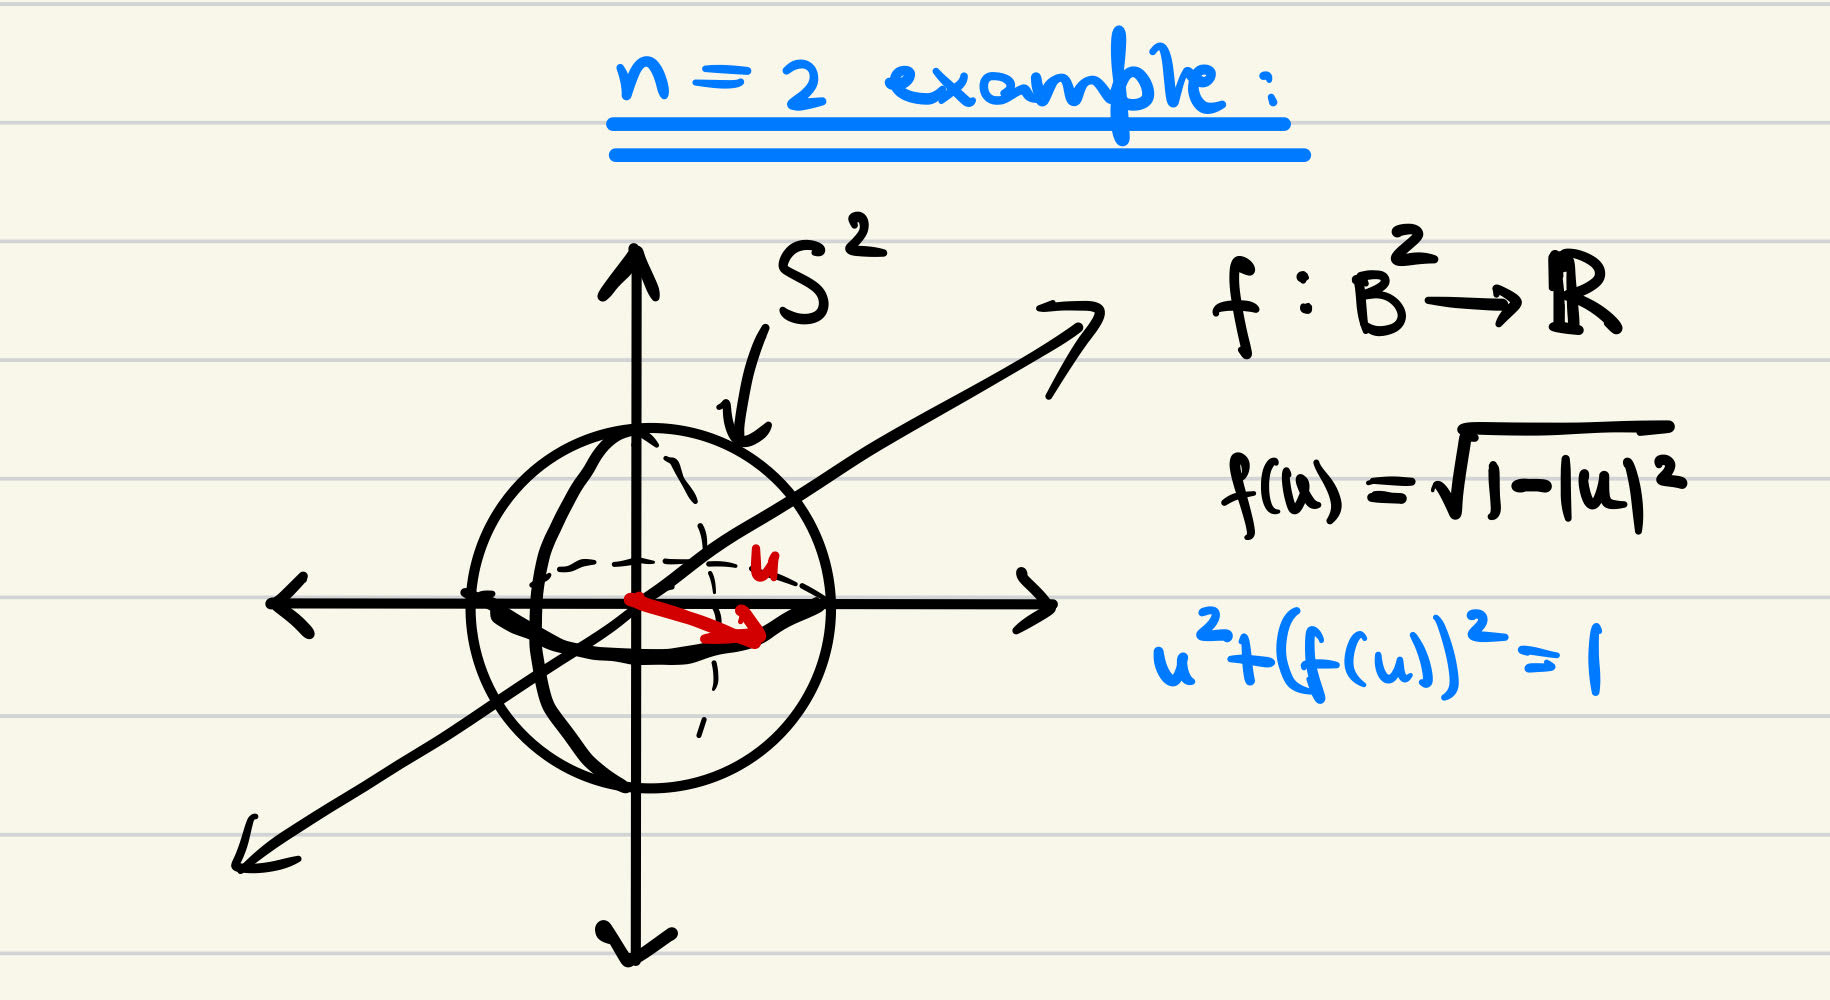
\includegraphics[scale=0.10]{Q11.jpg}
\end{center}

\vskip 0.5cm
Then, the set $U_i^{+} \cap \mathbb{S}^n$ is the graph of 
\[ x^i = f(x^1, \dots, \hat{x}^i, \dots, x^{n+1}) \]
where the hat above $x^i$ indicates that it is omitted, since 
\begin{align*}
  &x^i = 1 - \left[ (x^1)^2 + \cdots + (x^{i-1})^2 + (x^{i+1})^2 + \cdots + (x^{n+1})^2 \right] \\
  \implies &(x^1)^2 + \cdots + (x^{i-1})^2 + (x^i)^2 + (x^{i+1})^2 + \cdots + (x^{n+1})^2 = 1
\end{align*}

Similarly, the set $U_i^{-} \cap \mathbb{S}^n$ is the graph of 
\[ x^i = -f(x^1, \dots, \hat{x}^i, \dots, x^{n+1}) \]

Thus, each of the sets $U_i^{\pm} \cap \mathbb{S}^n$ is locally euclidean on dimension $n$. The coordinates on $\mathbb{S}^n$ are given by 
\[ \phi_{i}^{\pm}(x^1, \dots, x^{n+1}) = \pm f(x^1, \dots, \hat{x}^i, \dots, x^{n+1}) \]

Since each point on $\mathbb{S}^n$ must necessarily lie in one of the sets $U_i^{\pm} \cap \mathbb{S}^n$, each point lies in the domain of at least one chart. Hence, $\mathbb{S}^n$ is a topological $n-$dimensional manifold.

\vskip 0.5cm
\hrule 
\vskip 0.5cm

% \printbibliography

\end{document}
